\chapter{Method Description}

In this section, the origin DOI method, JDOI method and approximation method based on DOI method are described. In section \ref{sec: 2.1},, we introduce the origin DOI method. In section \ref{sec: 2.2}, we illustrate the approximation method proposed by \cite{kristensen_adding_2011}. In section \ref{sec: 2.3}, we discuss our estimator to price American options based on JDOI method.

\section{The DOI Variance Reduction Method}
\label{sec: 2.1}

Consider a multi-factor model, in which a $d$-dimensional vector of state variables $X(t)$ on a filtered probability space$(\Omega,\mathcal F, \mathbb Q)$ satisfies the following Stochastic Differential Equations(SDEs)

\begin{equation}\label{general model}
    dX(t) = \mu(t, X(t)) dt + \sigma(t, X(t)) dW(t)
\end{equation}

\noindent where $\mu(t,X(t))$ and $\sigma(t, X(t))$ are drift and diffusion functions under the risk-neutral measure $\mathbb Q$, which also satisfies appropriate growth and Lipschiz conditions such that equation(\ref{general model}) admits a unique strong solution and is Markovian; $W(t)$ is a $d$-dimensional standard Brownian Motion and $t \in [0,T]$.

% Besides, we also need to consider the stopping time formulation such that we can apply DOI method to path-dependent options, we shall discuss it later in section \ref{sec: 2.3} when pricing American options.

% Let $G(t, x)$ be the payoff function of derivatives written on $X(t)$ and current state $X(t) = x$, $t\in[0,T]$, assume $G(t,x)$ satisfies that 

% \begin{equation}
%     \mathbb{E}_{t, x}\left[\sup _{0 \leq u \leq T-t}\left|e^{-\int_t^{t+u} R(s,X(s)) ds} G(T, X(t+u))\right|\right]<\infty
% \end{equation}

% \begin{equation}
%     V(t,x) = \mathbb{E}^{t,x}[e^{-\int_t^T R(s,X(s)) ds} G(T, X(T))]
% \end{equation}

Let $V(t,x)$ be the value function of European option written on $X(T)$ with current state $X(t)=x$, $G(t, x)$ be the payoff function. We define the infinitesimal generator $\mathcal{L}$ associated with equation(\ref{general model})to be

\begin{equation}\label{general inf gen}
    \begin{aligned}
        (\mathcal{L} V)(t, x)&=\frac{\partial V}{\partial t} + \sum_{i=1}^{d} \mu_i(t, x) \frac{\partial V}{\partial x}+\frac{1}{2} \sum_{i=1}^{d}\sum_{j=1}^{d} (\sigma(t,x) \sigma^{\intercal}(t,x))_{i,j} \frac{\partial^2 V}{\partial x_i x_k}
    \end{aligned}
\end{equation}

Let $R(t,x)$ be the instantaneous short-term interest rate, $Q(t,x)$ the instantaneous coupon rate, combining with equation(\ref{general model}) and equation(\ref{general inf gen}), the price of European option $V$ is a solution to the following partial differential equation(PDE)

\begin{equation}
    LV(x,t) = (R(x,t) - Q(x,t))V(x,t)
\end{equation}
\noindent with boundary condition $V(T,x(T)) = G(T,X(T))$. It's easily seen that under risk neutral measure $\mathbb Q$, the instantaneous option price change is equal to the price gain in saving account minus paid coupon. 

Next we consider to use a $m$-dimensional($m \leq d$) process $\bar{X}(t)$ which is a simpler process to approximate the price of option. $\bar{X}(t)$ satisfies the following SDE

\begin{equation}\label{approx model}
    \begin{aligned}
        &d\bar{X}(t)= \begin{cases}   \bar{\mu}_i(t, \bar{X}(t)) dt + \bar{\sigma}_i(t, \bar{X}(t)) dW(t) & 1 \leq i \leq m \\
        0 & \text { otherwise }\end{cases}
        \end{aligned}
\end{equation}

\noindent where $\bar{\mu}(t, \bar{X}(t))$ and $\bar{\sigma}(t, \bar{X}(t))$ are drift and diffusion functions, and they are also assumed to satisfy appropriate conditions such that equation(\ref{approx model}) admits a unique strong solution and is Markovian.

With this new process, the European option written on $\bar{X}(t)$ is given by

\begin{equation}
    \bar{V} = \mathbb{E}_{t, x}\left[e^{-\int_t^{t+u} R(s,\bar{X}(s)) ds} G(T, \bar{X}(t+u))\right]
\end{equation}

\noindent and assume the following additional integrability condition

\begin{equation}
    \mathbb{E}_{t, x}\left[\sup _{0 \leq u \leq T-t}\left|e^{-\int_t^{t+u} R(s,\bar{X}(s)) ds} G(T, \bar{X}(t+u))\right|\right]<\infty
\end{equation}

Additionally, strong Markovian arguments imply that the European-style option $\bar{V}$ satisfies

\begin{equation}
    L\bar{V}(x,t) + q(t,x) = R(x,t)\bar{V}(x,t)
\end{equation}

It's easily seen that

\begin{equation}
    V(t,x) = \bar{V} + \mathbb{E}_{t,x}\left[\right]
\end{equation}

\section{Approximation Method based on DOI method}
\label{sec: 2.2}

\section{JDOI method}
\label{sec: 2.3}
  
\normalsize 

% \begin{figure}[htp]
% \centering
% 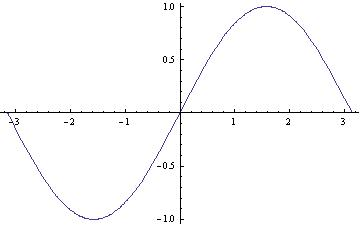
\includegraphics{sin_x.jpg}
% \caption{Transverse momentum distributions}\label{fig:erptsqfit}
% \end{figure}

